% !TEX root = ../../main.tex
\subsection{Task 2: Observation and Parameter Estimation}
\label{sec:task-2}

\subsubsection{Observation Model}

第 $n$ 周的报告新增预测及报告累计量分别为
\begin{align}
\widehat y_n&=\int_{n-1}^{n}\rho(t)\,\alpha\sum_{j,k}E_{jk}(t)\,\mathrm dt,
\label{eq:weekly-observation}\\
C^{\mathrm{rep}}(t)&=8+\int_0^t\rho(u)\dot C(u)\,\mathrm du.
\label{eq:reported-cumulative}
\end{align}
末周的积分上限取实际截止时间。周病例用于估计总体强度 $k(t)$ 与初始状态，病程参数和报告比例作为外部约束。

\subsubsection{Parameterization and Estimation}

在节点 $\tau_\ell$ 间对 $\log k(t)$ 作线性插值，最小化加权残差与节点二阶差分惩罚：
\begin{equation}
\begin{split}
\min\quad &\sum_{n=1}^{n_{\mathrm{obs}}}
\frac{(\widehat y_n-y_n)^2}{y_n+1}\\
&+\eta\sum_{\ell=2}^{L-1}
\left[\log k(\tau_{\ell+1})-2\log k(\tau_\ell)
+\log k(\tau_{\ell-1})\right]^2.
\end{split}
\label{eq:fitting-objective}
\end{equation}
$L$ 为节点数；病例以“1 例”为单位数值化，$\eta$ 为无量纲权重。采用有界非线性最小二乘，正值参数在对数尺度上估计，概率参数限于 $[0,1]$。多初值计算用于检验局部最优。

参考计算的全样本拟合使用 27 周数据和 16 个节点；时间回测仅用前 20 周及 11 个节点拟合，随后固定末节点强度预测第 21--27 周。评价指标为
\begin{align}
R^2&=1-\frac{\sum_n(y_n-\widehat y_n)^2}
{\sum_n(y_n-\overline y)^2},\notag\\
\mathrm{RMSE}&=\sqrt{\frac{1}{n_{\mathrm{obs}}}
\sum_n(y_n-\widehat y_n)^2},\qquad
\mathrm{MAPE}=\frac{100\%}{n_{\mathrm{obs}}}
\sum_n\frac{|y_n-\widehat y_n|}{y_n}.
\label{eq:fit-metrics}
\end{align}
$\overline y$ 为评价区间的观测均值，RMSE 以例计。当前周观测均为正，MAPE 无零分母。

\subsubsection{Fit and Temporal Validation}

根据所给参考预测序列重算得到表~\ref{tab:fit-audit}。全样本 $R^2=0.955$，但验证段 RMSE 为训练段的 3.61 倍，外推误差明显增加。

\begin{table}[!htbp]
\centering
\caption{参考预测序列的拟合与回测误差}
\label{tab:fit-audit}
\begin{tabular}{@{}lrrr@{}}
\toprule
评价区间 & $R^2$ & RMSE（例） & MAPE \\
\midrule
全样本拟合（1--27 周） & 0.955 & 34.61 & 6.90\% \\
回测训练段（1--20 周） & 0.969 & 33.09 & 6.96\% \\
回测验证段（21--27 周） & $-4.577$ & 119.50 & 20.15\% \\
\bottomrule
\end{tabular}
\end{table}

\begin{figure}[!htbp]
\centering
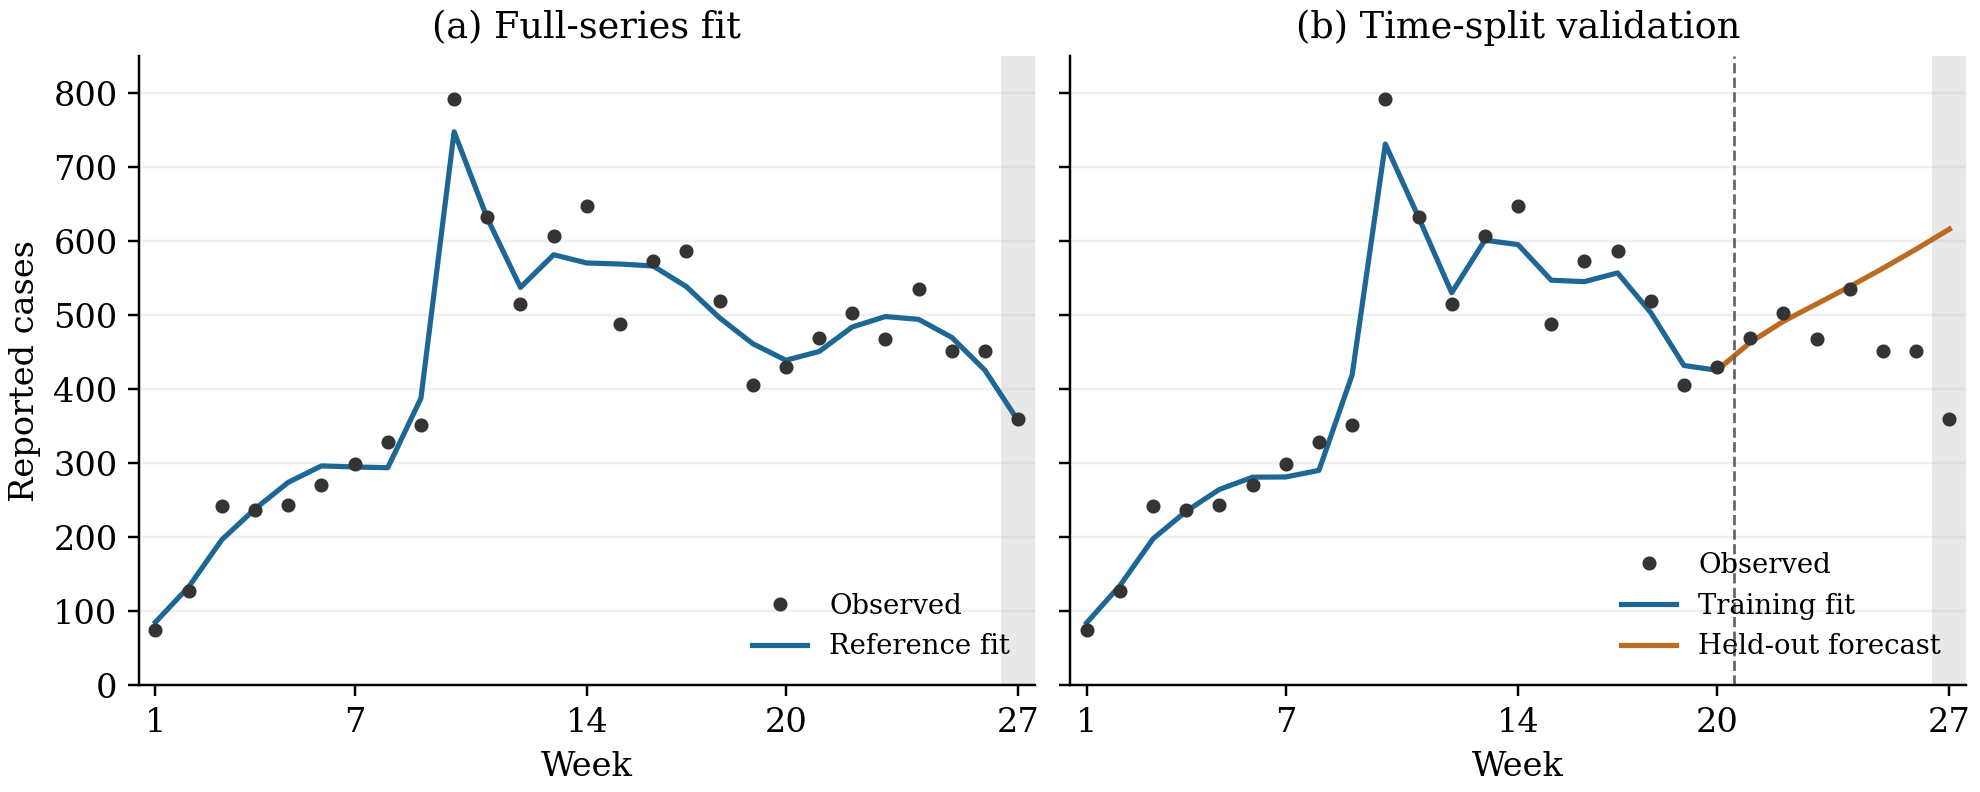
\includegraphics[width=0.94\linewidth]{model-fit-check.png}
\caption{参考计算的全样本拟合（左）与时间回测（右）；灰色区域为未完整覆盖的第 27 周，虚线为训练与验证分界。}
\label{fig:model-fit-check}
\end{figure}

全样本预测新增合计为 11\,517 例，观测合计为 11\,605 例。回测末周预测 616 例、记录 359 例；验证段 $R^2<0$，表明其平方误差超过以该段观测均值作常数对照的误差。末周覆盖及平滑权重的影响在第~\ref{sec:sensitivity} 节分析。
